\noindent
{\bf Collaborative research: Self-organization modeled by moving domain
elliptic PDEs} \\
{\em Rolf Ryham (PI, Fordham University),
Bryan Quaife (lead PI, Florida State University), and
Yuan-Nan Young (PI, New Jersey Institute of Technology)}

\section{Background}
\label{sec:background}

Self-organization encompasses a broad range of
interesting and challenging phenomena in engineering and science.
For example, understanding the
organization of lipids and proteins in vesicles is crucial to design
effective drug carriers
and functional mimics of cell membranes
\cite{Marui2022IncreasedEO,https://doi.org/10.1002/adma.202206288}.
The COVID-19 pandemic has led to a
concerted, worldwide efforts to understand
the mechanisms of RNA condensation by structural proteins protein
oligomerization that control virus structure
\cite{Kim2021SelfassembledMV}.
Engineers have developed superior techniques
that rely on nanoscale  
capillary and van der Waals forces
to print high-resolution
features on devices \cite{Zeng20223DprintedMT}.
Finally, researchers design efficient algorithms for
constructing for the interaction kernels to study complex
patterns in agent-based systems like swarms and flocking
\cite{Lu2019NonparametricIO,Tadmor2021OnTM}.

%A number of mathematical techniques have been developed to handle
%self-organizing systems. Each technique has its advantages and
%disadvantages. Prominent in chemistry and biology, molecular dynamics
%(MD) simulations offers unparalleled resolution of protein-lipid
%interactions, say, but because of the large number of non-linear
%interactions involved, is limited to short time and small spatial
%scales. In terms of inverse problems, agent based systems also involve
%relatively large numbers of particles and researchers extensively
%consider the problem of using trajectory data to learn interaction
%kernels of the dynamics when constrained to evolve on Riemannian
%manifolds. Once the interaction kernels are known, one can in principle
%derive partial differential equations (PDE) for the macroscopic
%behavior. 

When fluids are involved,
tracking self-organization
becomes difficult due to the deformability of
suspended media.  A dominant approach in this area,
the phase field method
introduce a scalar-valued phase
field function for the volume fraction of
amphiphilic lipids or polymers in solvent, for example.
Sometimes called diffuse interface
methods, one devises energy functionals involving the gradient and
well-potentials of the phase field, and possibly long range interaction
kernels, 
\cite{Promislow2022UndulatedBI,C9SM01983A,doi:10.1063/5.0009734,
LiAn-Chang16,Choksi2003OnTD}.
Because the fluid interfaces are given by the
level-set of a smooth function,
they can have almost arbitrary topology
e.g., free ends, junctions
\cite{Promislow2017ExistenceBA,Promislow2022UndulatedBI},
the evolution equations can be studied
by well-established tools variational and analytical means,
\cite{Gavish2011CurvatureDF,Dai2019WeakSF,Dai2015CompetitiveGE,
Dai2022GeometricEO,Dai2020MinimizersFT,Dai2013GeometricEO},
and the governing equations are amenable to numerical approximation
\cite{Christlieb2020BenchmarkCO,Christlieb2019CompetitionAC}.
One of the downsides, though, 
is that granular details like molecular orientations and
shape changes induced by proteins that may be crucial to the physics, are
clumsy to incorporate in the model. Moreover, numerical simulations of
phase field models typically discretize the entire fluid domain under
consideration, and apply cutoff boundary conditions when periodic
domains are not under consideration. 

\begin{figure}
  \begin{center}
%    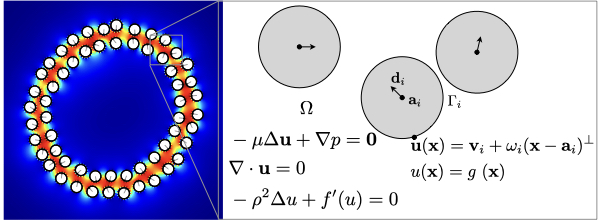
\includegraphics[width=0.45\textwidth]{figures/SpecificAim1/Domain.jpg}
%    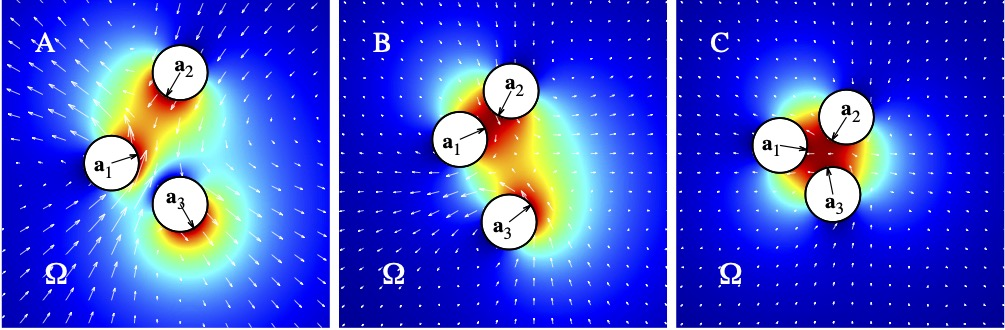
\includegraphics[width=0.45\textwidth]{figures/SpecificAim1/3Particles.jpg}
    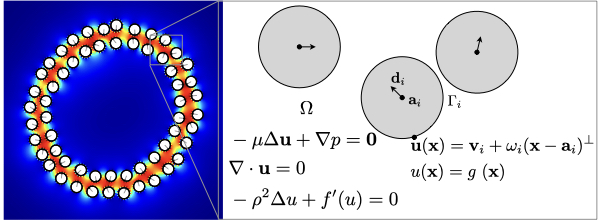
\includegraphics[keepaspectratio,height=2.7cm]{figures/SpecificAim1/Domain.jpg}
    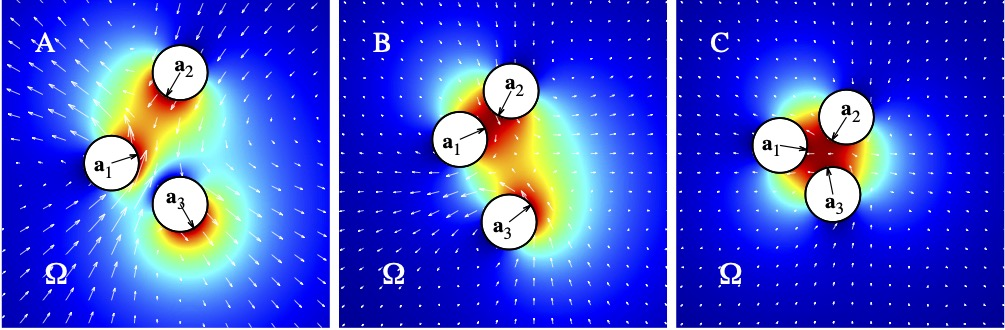
\includegraphics[keepaspectratio,height=2.7cm]{figures/SpecificAim1/3Particles.jpg}
  \end{center}
  \caption{\label{fig:flow_map} \footnotesize {\em Left:} In the HAP
  formulation~\cite{Fu2018_SIAM}, a system of exterior problems defines
  the hydrodynamic and hydrophobic interactions. {\em Right:} Particles
  translate and rotate to lower the free energy $E[u]$ subject
  to~\eqref{eqn:phase}, $W(\phi) = \phi^2$, and reach a minimal
  configuration in panel C. The colormap is blue for $\eta = 0$ and red
  for $eta = 1$. The arrows are the velocity field $\uu$.}
\end{figure}

\subsection{Problem formulation}
We recently developed a new mathematical model of
self-organization~\cite{FuQuRyYo22,fu-ryh-qua-you2022,Fu2018_SIAM}.
It takes ideas from the phase field method and leverages boundary
integral equations to resolve complex domains and speed up computations.
To formulate the problem, consider a collection of $N_b$-many rigid
bodies $U_i(t) \subset \RR^n$ with boundary $\Gamma_i(t)$. We call these
bodies ``granules''. The granules are immersed in an incompressible,
zero-Reynolds number fluid $\Omega(t) = \RR^n \setminus \cup_{i=1}^{N_b}
U_i(t)$ (Figure~\ref{fig:flow_map}).
Throughout, $\nnu$ refers to unit
normal pointing into $\Omega(t)$ (Figure~\ref{fig:flow_map}).

To determine how the granules move through space,
we look for rigid body transformations
\begin{align}
\label{eq:RBT}
  F_i(\XX,t) = R_i(t)(\XX - \aa_i(0)) + \aa_i(t),\quad \XX \in U_i(0),
\end{align}
where $i = 1,\ldots,N_b,$ $R_i(t)$ is a rotation (proper orthogonal) $n
\times n$ matrix, $\aa_i(t)$ are the granule centers, and $\XX$ is a
reference coordinate.
The dynamics come from the following system of semi-linear, elliptic boundary value problems:
\begin{alignat}{4}
  \label{eqn:stokes} 
  -\mu\Delta \uu + \nabla p &= \mathbf{0}, 
  \quad \nabla \cdot \uu = 0, &&\xx \in \Omega(t), \\
  \label{eqn:phase}
  -\epsilon^2 \Delta \phi + W'(\phi) &= 0, &&\xx \in \Omega(t),\\
  \label{eqn:noslip}        
  \frac{dF_i}{dt}(\XX,t) & = \uu(\xx) = 
    \vv_i + \omega_i \times (\xx - \aa_i), 
  \quad &&\xx \in \Gamma_i(t),\\
  \label{eqn:material}
  \phi(\xx) &= h_i(\XX),  &&\xx \in \Gamma_i(t),
\end{alignat}
for $i=1,\ldots,N_b$ and where $\xx = F_i(\XX,t)$.  Finally,
\begin{align}
\label{eqn:stressbalance}
\int_{\Gamma_i} \left(\sigma  + T_i\right)\nnu \,\dif s = \mathbf{0},\quad
\int_{\Gamma_i} (\xx - \aa_i)\times \left(\sigma + T_i\right) \nnu \,\dif s = \mathbf{0}
\end{align}
where
\begin{align}
\label{eqn:hydro_stress}
\sigma = \mu(\nabla \uu + \nabla \uu^T) - pI,\quad 
T_i = \gamma\left[\epsilon^{-1} W'(\phi)I
  + \epsilon\left(\tfrac{1}{2}|\nabla \phi|^2I - \nabla \phi \nabla
  \phi^T\right)\right]
\end{align}
are the hydrodynamic and phase field stresses, respectively.
Equation~\eqref{eqn:stokes} is the Stokes equations 
describing the velocity $\uu$ and pressure $p$ of the aqueous region with
viscosity $\mu$.
Equation~\eqref{eqn:phase} describes the
transitions of the scalar order parameter $\phi$ with a decay length
$\epsilon$.
The scalar function $W(\phi) : \mathbb{R} \to \mathbb{R}$ is a nonnegative
well-potential with local minima $\phi_0, \phi_1$  etc.
representing metastable states of the solvent.
For the single well case, $W(\phi) = \frac{1}{2}\phi^2$
has the minimum $\phi_0 = 0$ and the phase field equation
\eqref{eqn:phase} becomes the \emph{linear} screened Laplace equation.
For the double well case e.g, $W(\phi) = \frac{1}{4}(\phi^2-1)^2+cx$, $c > 0$,
the phase field equation \eqref{eqn:phase} takes the form of an
Allen-Cahn equation with local minima $\phi_0 < 0 < \phi_1$.
Section \ref{sec:specificaim1} discusses certain
modifications needed for \eqref{eqn:phase} in the nonlinear case.

For the moving domain boundary conditions,
equations~\eqref{eqn:noslip} specify a no-slip boundary condition for a
rigid body with translation velocity $\aa'_i(t) = \vv_i$ and angular
velocity $\omega_i$ (the axial vector for $R'_i(t)R_i(t)^T$)
about the point $\aa_i(t) \in U_i(t)$. In
equation~\eqref{eqn:material}, the function $h_i$ is a material label
specifying the phase at water-granule interface.
Finally, equation~\eqref{eqn:stressbalance} closes the system by requiring that
the force and torque generated by hydrodynamic stress balances that
generated by phase stress $T_i$ in~\eqref{eqn:hydro_stress}. The
parameter $\gamma > 0$ is surface tension,
$I$ is the $n\times n$ identity matrix,
and we define the ``cross product'' as
$\aa \times \bb = (\aa^{\perp} \cdot \bb) \kk$ where $\kk = (0,0,1) \in
\RR^3$ and $(a_1,a_2)^{\perp} = (-a_2,a_1)$ when $\aa, \bb \in \mathbb{R}^2$.


We call the rigid bodies $U_i(t)$ granules since they are small, compact
parcels of a suspended media, e.g.~lipids, Janus spheres. We use the
shape and boundary conditions for $U_i$ to capture the local properties
of the suspended media. We have departed from the terminology
``particles'' to emphasize the role played by their finite size. In our
simulations (see \S\ref{sec:specific_aim1}), we include a finite length
repulsion to avoid particle collisions.

\begin{wrapfigure}[]{l}{2.1in}
  \centering
  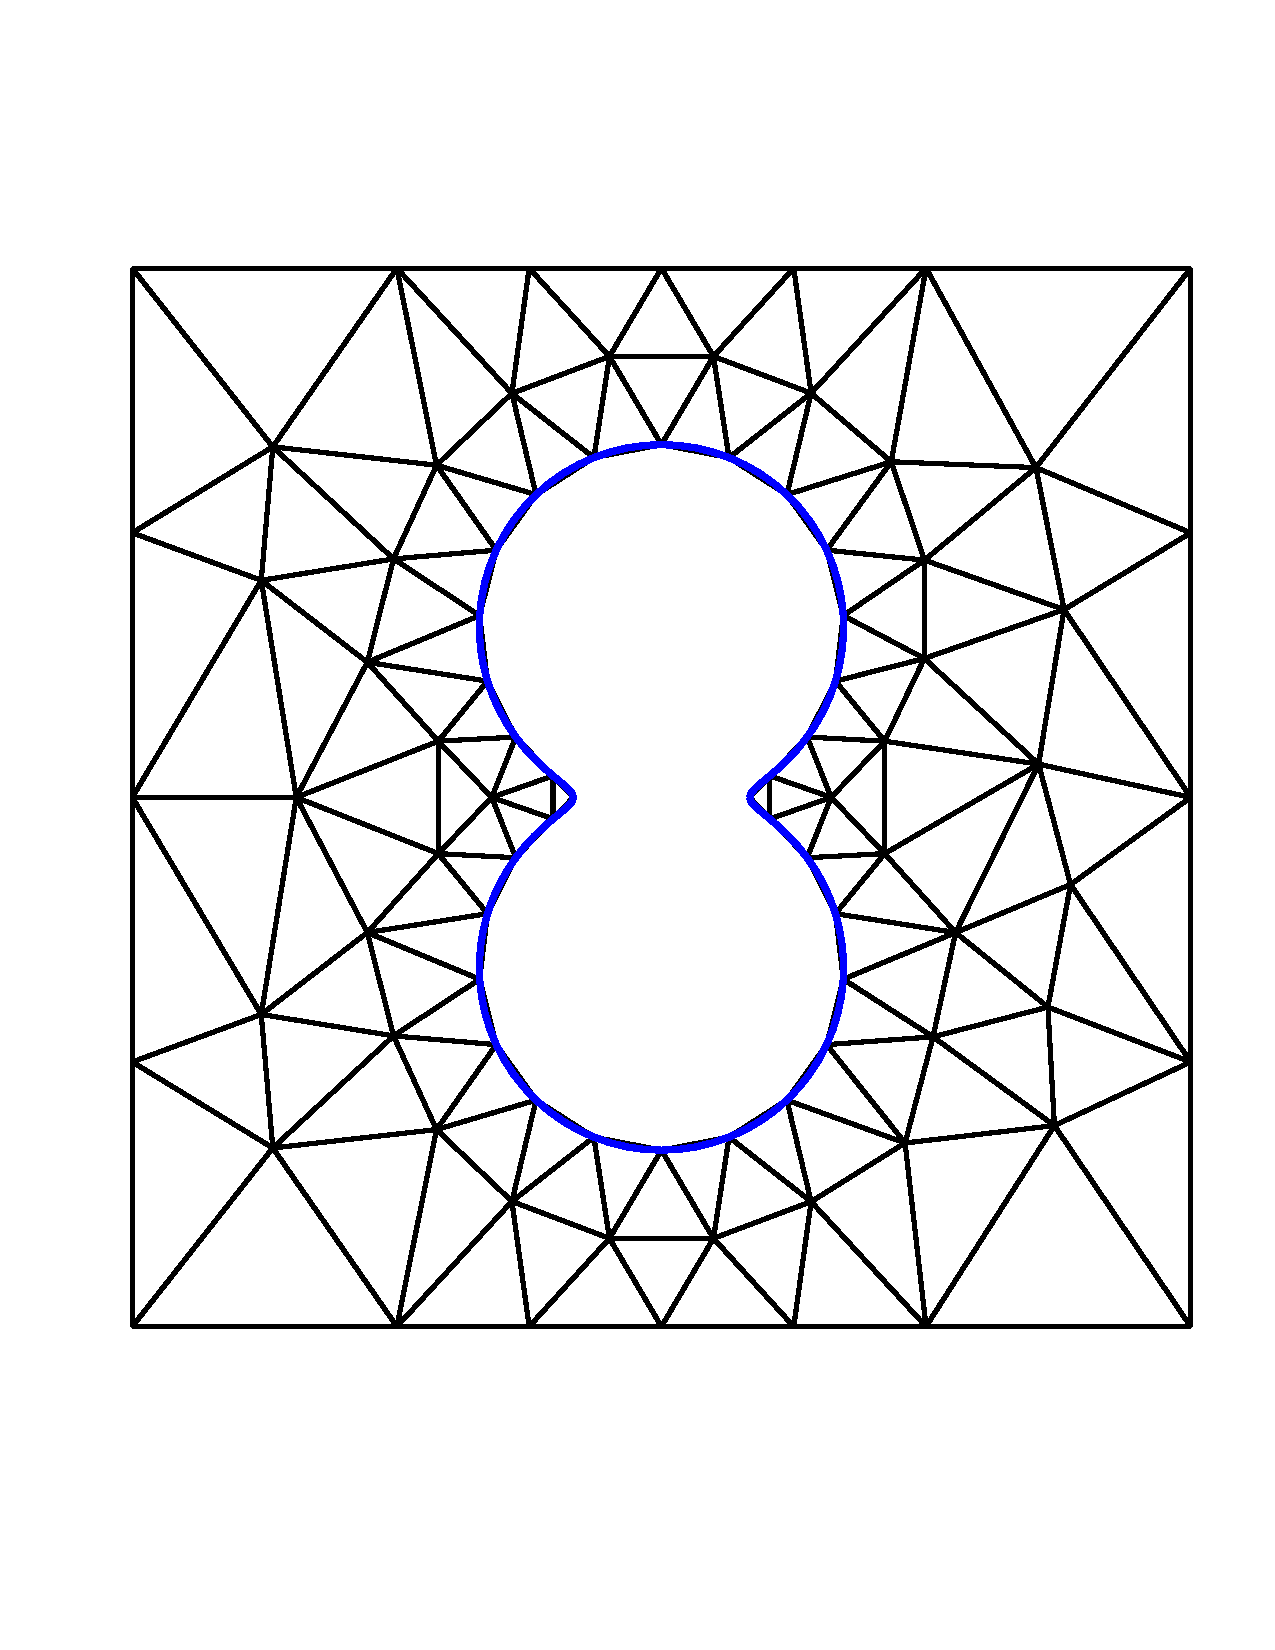
\includegraphics[width=1in]{figures/Background/Peanut/PeanutFEM.pdf}
  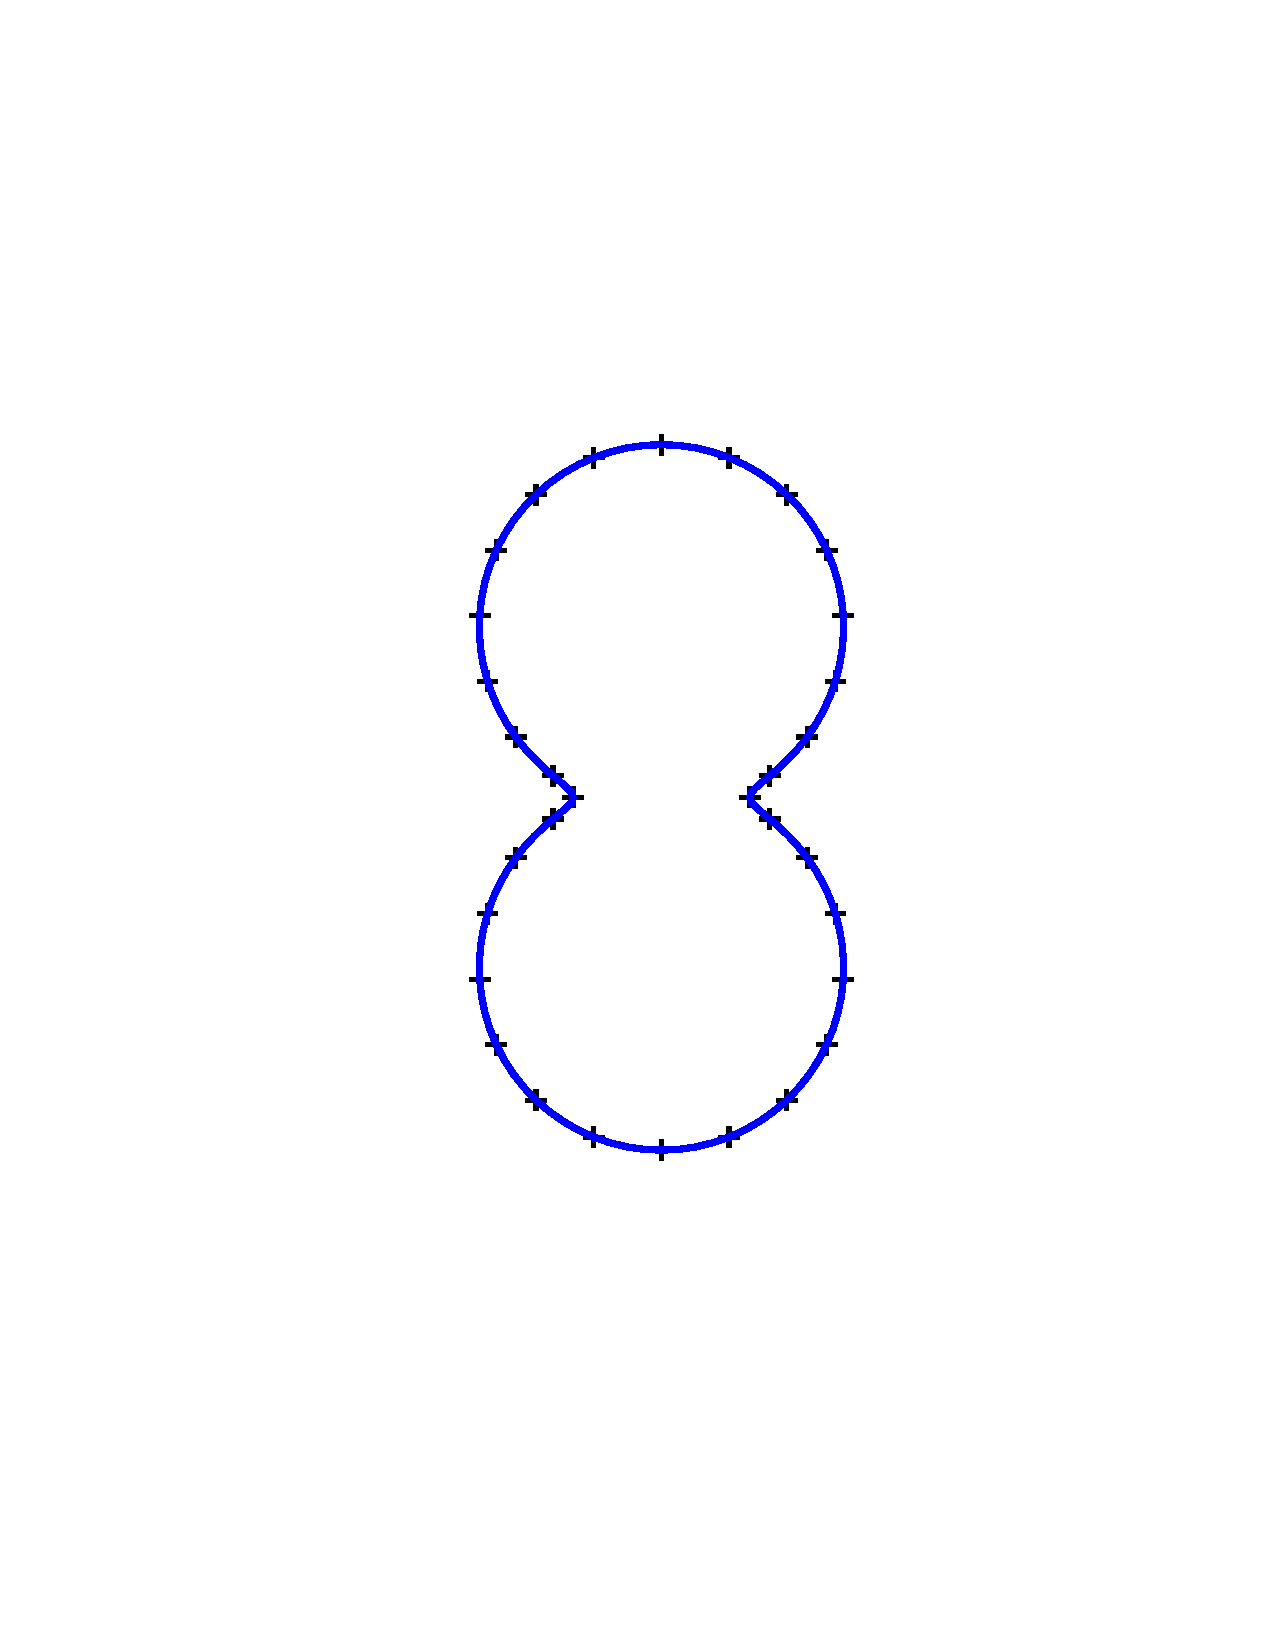
\includegraphics[width=1in]{figures/Background/Peanut/PeanutIE.pdf}
  \caption{\label{fig:fem_vs_bie} \footnotesize A finite element method
  ({\em left}) requires meshing the entire domain (typically into
  triangles), while a BIE ({\em right}) requires meshing only the
  boundary of the domain.}
\end{wrapfigure}

Computational methods to solve the PDEs~\eqref{eqn:stokes}
and~\eqref{eqn:phase} are challenging to develop because of
the complicated and unbounded domain.
This challenge is compounded when dense
suspensions are considered. Integral equations (IEs) offer an
alternative formulation of the PDEs that only require meshing the
boundary of the granules rather than all of $\Omega(t)$
(Figure~\ref{fig:fem_vs_bie}), and the automatically satisfy far field
conditions. Additional advantages of an discretizations of IE
formulations include high-order, or even spectral, accuracy and
well-conditioned linear system that can be solved iteratively with a
mesh-independent number of Krylov iterations such as the generalized
minimal residual method (GMRES). However, IEs have challenges: nearly
touching granules requires a quadrature rule for nearly-singular
integrals; their discretization results in dense matrices; and they
cannot immediately be applied to non-linear PDEs. The IE community,
including PI Quaife, has developed a variety of tools to address these
numerical challenges, and we discuss our planned approach in
Section~\ref{sec:specificaim2}.

In the absence of external flow, the
system~\eqref{eq:RBT}--\eqref{eqn:stressbalance} has the energy law
\begin{align}
\label{eq:energy_law}
  \frac{d}{dt}E
  = - \int_{\Omega(t)}\tfrac{1}{2}\mu|\nabla \uu + \nabla
  \uu^T|^2 \,d\xx,\quad
    E = \gamma \int_{\Omega(t)}
  \frac{\epsilon}{2} |\nabla \phi|^2 + \frac{1}{\epsilon} W(\phi) \,d\xx.
\end{align}
Here $E$ is the energy stored in the phase transitions
and the energy law states that
the granules move to decrease energy,
which is lost due to viscous dissipation.
The derivation of \eqref{eq:energy_law} is interesting
because $E$ depends both on $\phi$
and $\Omega(t)$. It uses the Rayleigh Transport Theorem to write the time
derivative of $E$ as an energy density flux through the boundary
involving the phase stress $T_i$, and a bulk term involving the Euler-Lagrange
derivative of $E$~\cite{Fu2018_SIAM}. The Euler-Lagrange derivative vanishes due
to~\eqref{eqn:phase} and the boundary flux transforms into viscous
dissipation due to~\eqref{eqn:hydro_stress} and the Stokes equations. 

In the far field, $\lim_{\xx \to \infty} \phi(\xx) = \phi_0$ and for the
background flow, we require that $\lim_{\xx \to \infty} \uu(\xx) -
\uu_{\infty}(\xx) = \mathbf{0}$, where
the background flow takes the form
%In the case of shear background flow,
%for example,
%\begin{align}
%\label{eqn:shear_BG_flow}
%\uu_{\infty}(\xx) = \dot{\gamma} \xx \cdot \mathbf{e}_y \mathbf{e}_x,
%\end{align}
%where $\dot \gamma$ is the shear rate and $\mathbf{e}_x$, $\mathbf{e}_y$
%are horizontal and vertical basis vectors, respectively.
%Other
%background flows include
shear, extensional, parabolic Poiseuille, and
Taylor-Green flow, for example.
For numerical stability and physical realism, we
include pairwise repulsive forces and torques
in~\eqref{eqn:stressbalance} to prevent the collision between
neighboring granules which introduces a repulsive potential in the energy
law~\eqref{eq:energy_law}. Background flow adds elastic energy to the
granule configurations.
%and is quantified by simulation. We refer to the
%PIs work~\cite{FuQuRyYo22, fu-ryh-qua-you2022, Fu2018_SIAM} for details. 

In terms of physical justification, the derivation of the
one-dimensional version of our model was carried out using a Landau
expansion of the free energy density for a single-well
potential~\cite{MaRa76, ErLjCl89}. The double-well potential case was
considered by Gompper~\cite{GoHaKo94} to describe metastable
coordination of water. In the field of surface
chemistry~\cite{Israelachvili1954}, there is a large empirical
literature on properties of long-range hydrophobic
interaction~\cite{LeRaPa77, KoNa15, Nagle17, Lum1999, Lin2005,
Meyer2006, Ducker2016, Jackson2016, Gletal88, Aketal17, Ch05}. The
stress~\eqref{eqn:stressbalance} was first identified by PIs Ryham and
Young in~\cite{Fu2018_SIAM} and generalizes one-dimensional hydrophobic
interaction to the $n$-dimensional setting. 

In terms of mathematical justifications, we mention that when
equation \eqref{eqn:phase} takes the form of a screened Laplace equation
$-\epsilon^2 \Delta \phi + \phi =0$, for a fixed domain $\Omega$ with
smooth boundary, if the material label $h_i = 1$
everywhere, then $\phi$ has a boundary layer going from $1$ at the
boundary to $0$ in the bulk and one can prove that 
$\lim_{\epsilon \to 0} E = \frac{1}{2}\gamma |\partial \Omega|$.
In other words, because of the introduction of granule boundaries,
interfacial energy enters the problem even in the linear case.
We are confident
that~\eqref{eq:RBT}--\eqref{eqn:stressbalance} is a correct description
of long-range interactions between granule surfaces.

\begin{wrapfigure}[23]{r}{3.2in}
  \vspace{-15pt}
  \begin{center}
    \begin{tabular}{m{0.9in}m{0.9in}m{0.9in}}                 
    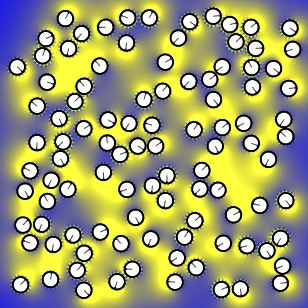
\includegraphics[width=0.85in]{figures/SpecificAim1/N100B1.jpg}
    &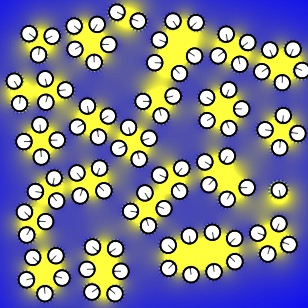
\includegraphics[width=0.85in]{figures/SpecificAim1/N100B2.jpg}
     &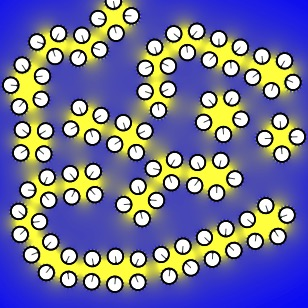
\includegraphics[width=0.85in]{figures/SpecificAim1/N100B3.jpg}    \\
    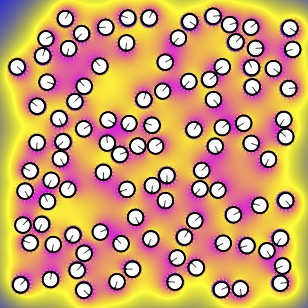
\includegraphics[width=0.85in]{figures/SpecificAim1/N100C1.jpg}
    &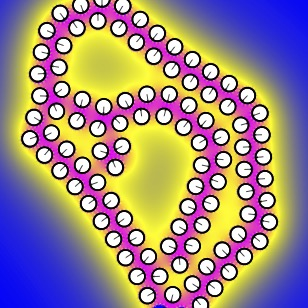
\includegraphics[width=0.85in]{figures/SpecificAim1/N100C2.jpg}
      &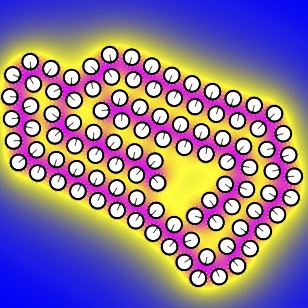
\includegraphics[width=0.85in]{figures/SpecificAim1/N100C3.jpg}    \\
      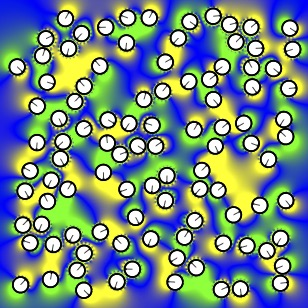
\includegraphics[width=0.85in]{figures/SpecificAim1/N100A1.jpg}
      &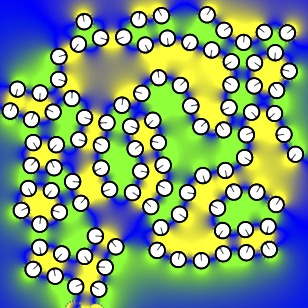
\includegraphics[width=0.85in]{figures/SpecificAim1/N100A2.jpg}
      &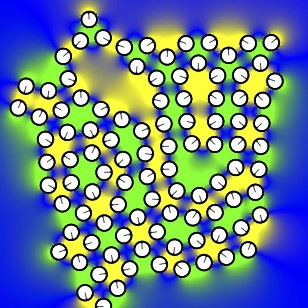
\includegraphics[width=0.85in]{figures/SpecificAim1/N100A3.jpg} 
  \end{tabular}
  \end{center}
  \vspace{-5pt}
  \caption{\footnotesize \label{fig:self-assembly2} Rows (a)--(c) have
  the same initial configuration but different boundary conditions $g$.
  {Top Row:} Granules with an amphiphilic boundary condition
  results in a bilayer pattern shielding the hydrophobic core (yellow,
  $\eta > 0$) from the aqueous phase (blue, $\eta = 0$). {\em Middle
  Row:} Biased granules with a hydrophobic intensity that is greater on
  one side of the particle (magenta) than the other (yellow). {\em
  Bottom Row:} Bipolar granules where green is for $\eta < 0$, yellow is
  for $\eta > 0$, and blue is for $\eta = 0$. Particles orient like
  sides to form a checkerboard pattern.}
\end{wrapfigure}

\subsection{Applications}
Since the formulation is scale independent, it can be applied broad
range of nonspecific self-organization phenomena in surface chemistry,
biology and engineering. For one, the
formulation~\eqref{eq:RBT}--\eqref{eqn:stressbalance} captures exactly
the right behavior expected from amphiphilic self-assembly.
For example,
three bodies with amphiphilic label (\S\ref{sec:specific_aim1})
spontaneously self-organize to sequester the hydrophobic fluid phase
(the red phase in Figure~\ref{fig:flow_map}).
Moreover, a simple change
of boundary conditions from amphiphilic,
to biased hydrophobic, to polar
results in distinct equilibrium morphologies
(Figure~\ref{fig:self-assembly2}).
Further applications include
(i) amphiphilic Janus spheres that form diverse suprastructures
\cite{HaBr20,McBr21,Bradley2017},
(ii) pickering emulsions involving
two-phase fluids and dense suspensions \cite{Bradley2016},
(iii) creation and manipulation of small droplets
using amphiphilic microparticles \cite{Ha2022SurfaceEM,Ha2020MinimalSC},
and (iv) tension drivent fabrication of microstructures
~\cite{Dasgupta2017, Leong2007, Reynolds2019, Cho2010,Zeng20223DprintedMT,Russell2016EnergyLF}.



\subsection{Vesicles as self-organized granules}
\label{sec:vesicles_as_granules}
Interface problems coming from biology are a challenging
area of applied mathematics.  Broadly speaking, these problems
involve a fluid structure interaction where the modeler must
solve for the velocity in the aqueous phase, track the interface,
and couple the velocity boundary condition to the interface through
stress balance boundary conditions.  The aqueous phase can
be a low Reynolds-number fluid, a porous medium, or viscoelastic fluid,
and the interfacial forces can come from surface tension, elasticity,
or electrostatics.
Incorporating all these details can lead to models with substantial
complexity and there is a need for robust, general models that
cut across these issues. 

This section shows the principles of PDE-driven
self-organization apply to the concrete
problem of \emph{vesicle hydrodynamics}.
A vesicle is a small, fluid filled membrane sack.
Microscopically, the membrane of a vesicle is comprised
elongated amphiphilic lipids that form inner and outer monolayers.  
The goal in vesicle hydrodynamics is to study the flow patterns e.g.,
tank-treading, tumbling, that arrise due to the interaction
between membrane elasticity and surrounding fluid.

There are downsides to traditional models in terms of generality and physical realism.
(i) Motivated by drug delivery applications, experimenters use electric
fields, for example, to controllably open and close pores in membranes
\cite{}.
These kinds of topological changes are clumsy to incorporate in
sharp interface formulations that assume a continuous surface \cite{}.
(ii) Sharp-interface models assume a membrane of neglible thickness. 
However, in biological processes
like fusion, fission, or insertion and penetration by proteins and peptides, 
the length scales of the
deformation (tens of nanometers) are comparable to membrane thickness (about 5 nm).
Moreover, these processes crucially rely on variable lipid
orientation relative to the surface normal (the so-called \emph{tilt}
deformation),
whereas \eqref{eq:Canham-Helfrich} implicitly assumes that the lipids
are everywhere normal to the surface.  
(iii) Finally, realistic membranes are comprised of a mixtures of lipids and proteins.
Recent work \cite{} has incorporated lipid mixtures in \eqref{eq:Canham-Helfrich},
but these models are formidably complicated 
due to the additional constraints and transport equations involved.

\begin{wrapfigure}[12]{r}{0.5\textwidth}
  \vspace{-5pt}
\centerline{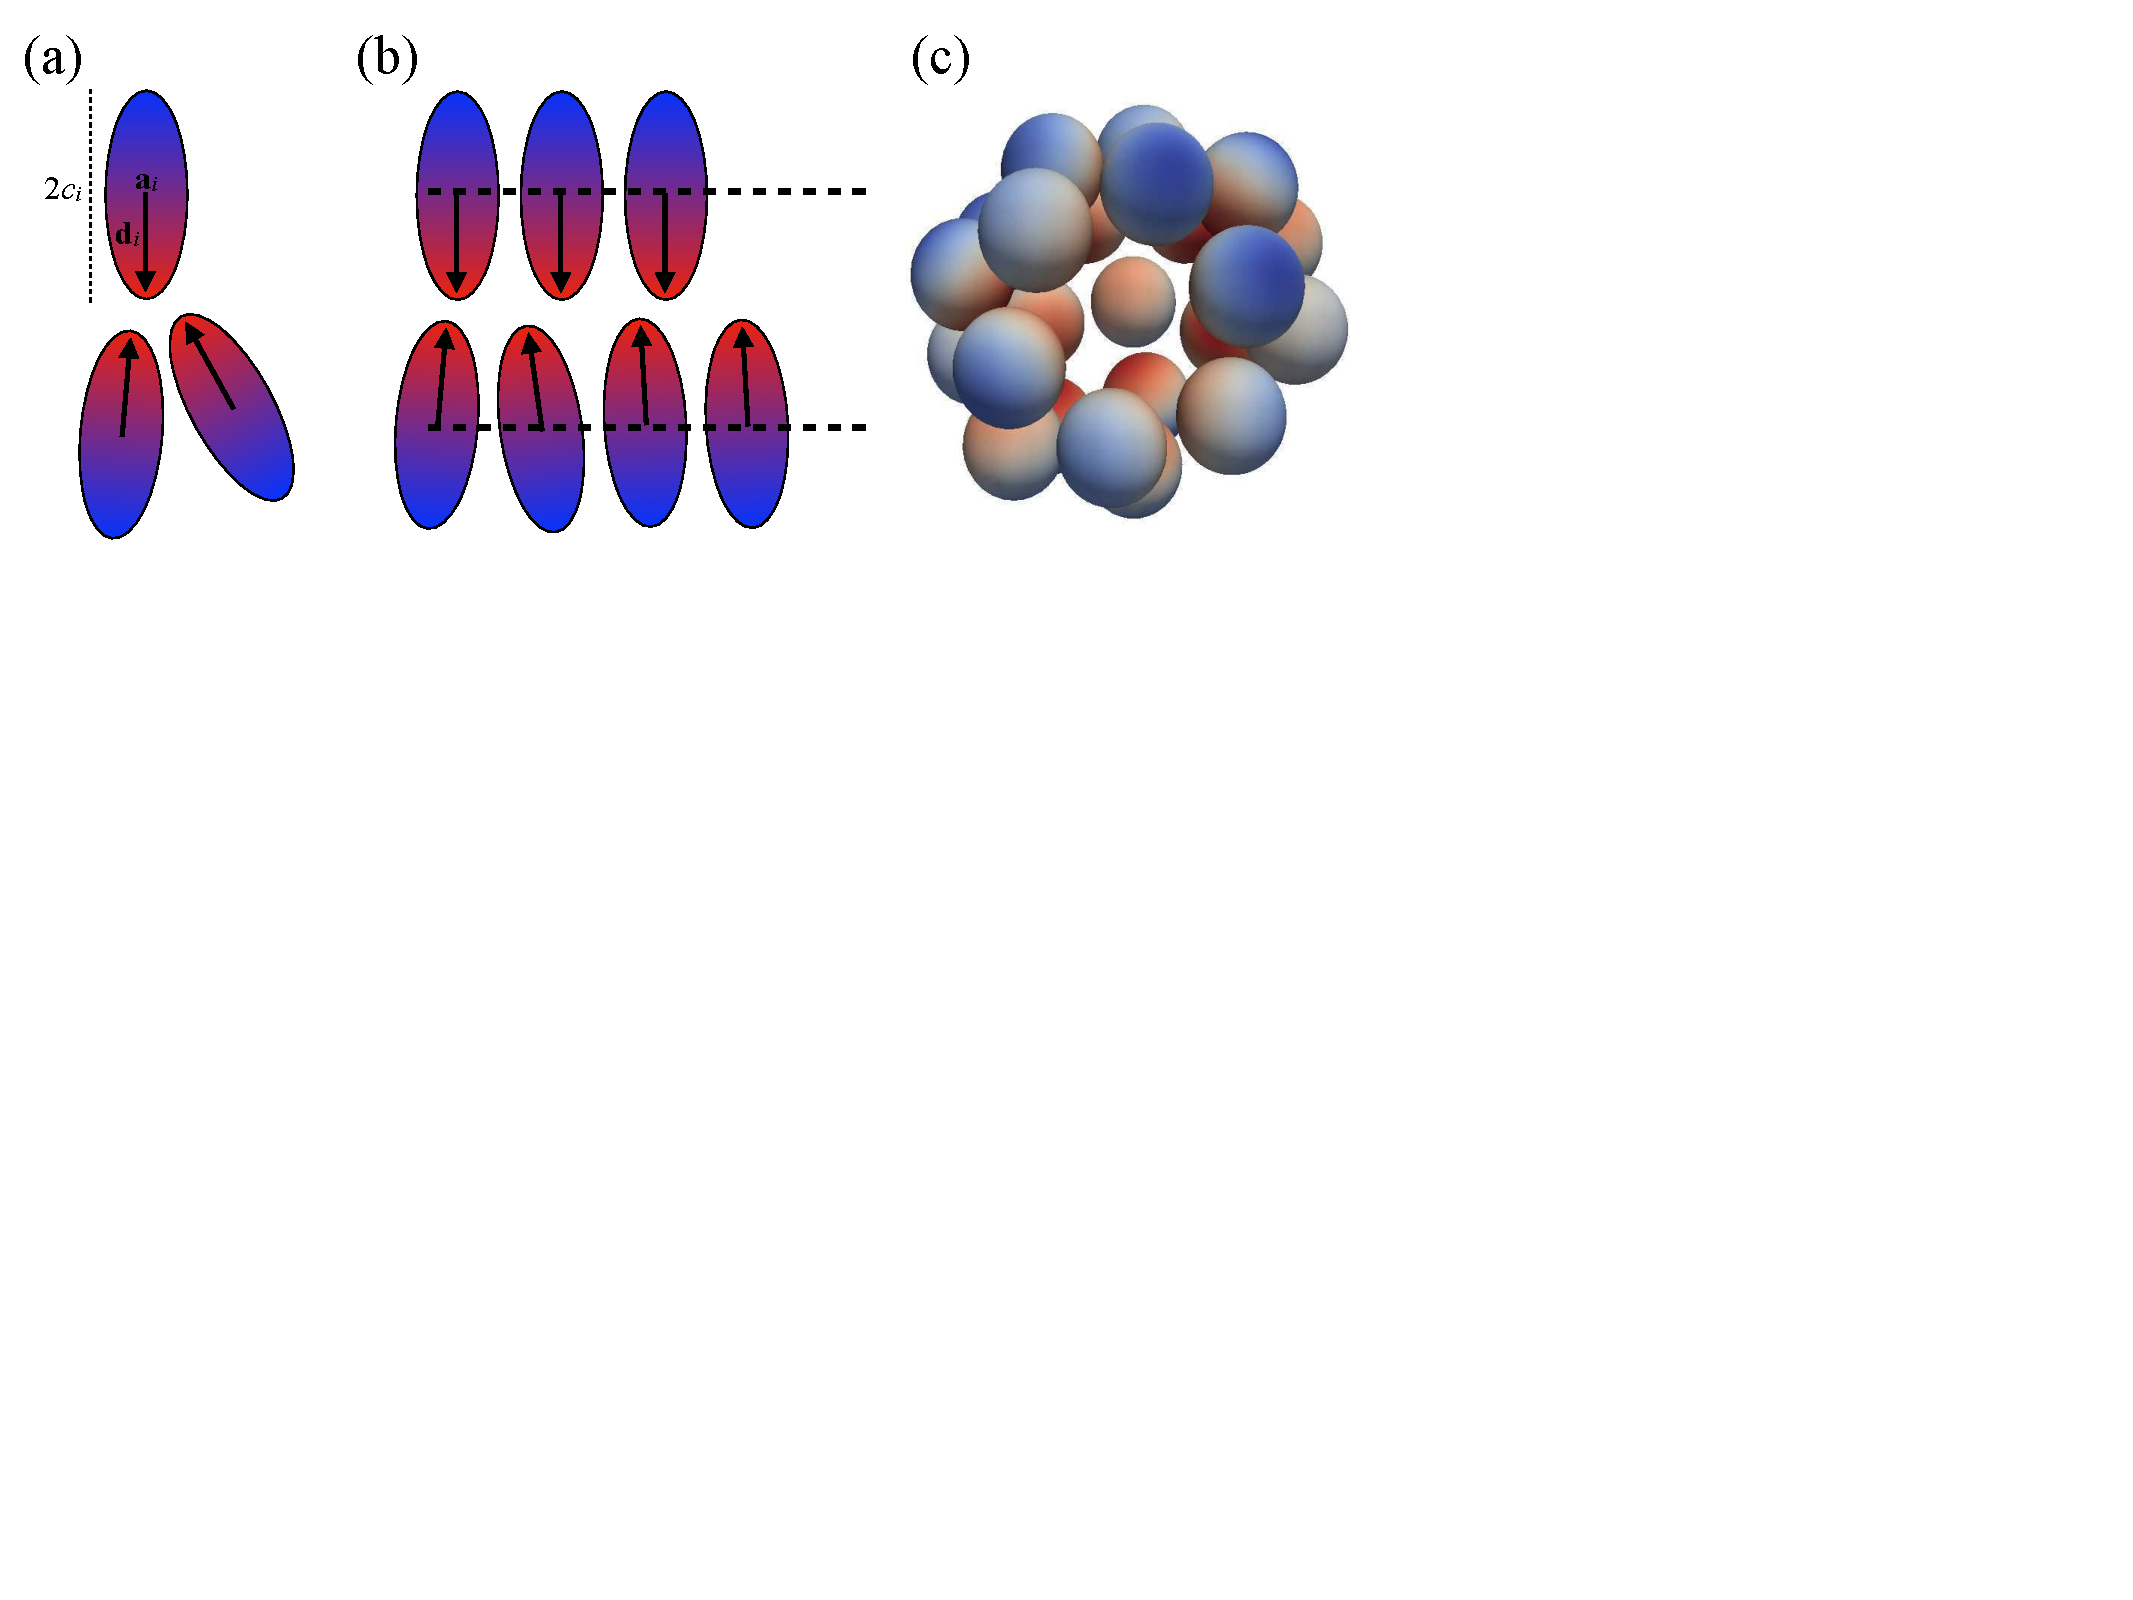
\includegraphics[width=0.5\textwidth]{figures/SA1Figures/AmphiphilicAssembly.pdf}}
  \vspace{-5pt}
\caption{\label{fig:amphiphilic_assembly}
Self-organization under amphiphilic boundary condition.
(a) Granules first match hydrophobic tails (red),
(b) then align length-wise.
The principle of self-organization holds in three dimensions 
as simulated by Kohl, Corona, and Veerapaneni
\cite{koh-cor-che-vee2021}.}
\end{wrapfigure}
Diffusive interface models and surface-director models partially address 
these shortcomings. 
Topological changes are permitted in phase field and level set formulations,
but these methods smear out the details of lipid orientations.
The detailed energies of lipid orientation that include tilt are
closely related to the celebraated and well-studied
field of nematic liquid crystals.  Here, there have been recent development
in simulation and theory of nematic liquid crystals on surfaces.
These models consider the interplay between defects and surface geometry \cite{},
finite element formulations \cite{}, and existence of minimizers \cite{}.

\subsubsection{Main modeling innovations}
We developed the model \eqref{eq:RBT}-\eqref{eqn:hydro_stress} 
as a robust and flexible approach
that cuts across many of the aforementioned challenges.
(i) The granules are not fixed to a stencil, 
affording flexibility in terms of vesicle morphology and topology--sufficiently
large forces will even pull the granules apart as physically required.
(ii) The model formulation is built around important details like lipid orientations,
and exhibits inter-monolayer slip that must be added into diffusive interface models
post hoc. 
(iii) It is straightforward to consider mixtures of granules with different
types of shapes and boundary conditions of the granules.
With the help of boundary integral equations
and fast summation methods, the dynamics can be solved in 
near-linear complexity in $N_b$, which is equal to or better than 
the computational complexity of related sharp interface methods. 

Inspired
by the amphiphilic structure of lipids,
we formulated a so-called
``amphiphilic'' boundary condition
that leads a collection of granules to form bilayers.
Referring to Figure \ref{fig:amphiphilic_assembly}, 
\begin{equation}
\label{eq:amphiphilic_BC}
\phi(\mathbf{x}) = h_i(\mathbf{x}) = \tfrac{1}{2}\left(\dd_i \cdot (\xx - \aa_i)/c_i + 1\right), \quad
\mathbf{x} \in \Gamma_i,
\end{equation}
where $\dd_i$ is the director, $\aa_i$ is the center, and $c_i$ the
``radius'' of the $i$th granule.  
The phase $\phi$ takes values close to $1$ on in the direction $\dd_i$,
representing a hydrophobic tail, and values close to $0$ 
in the direction $\dd_i$ representing the hydrophilic head.

\begin{figure}[t!]
\begin{center}
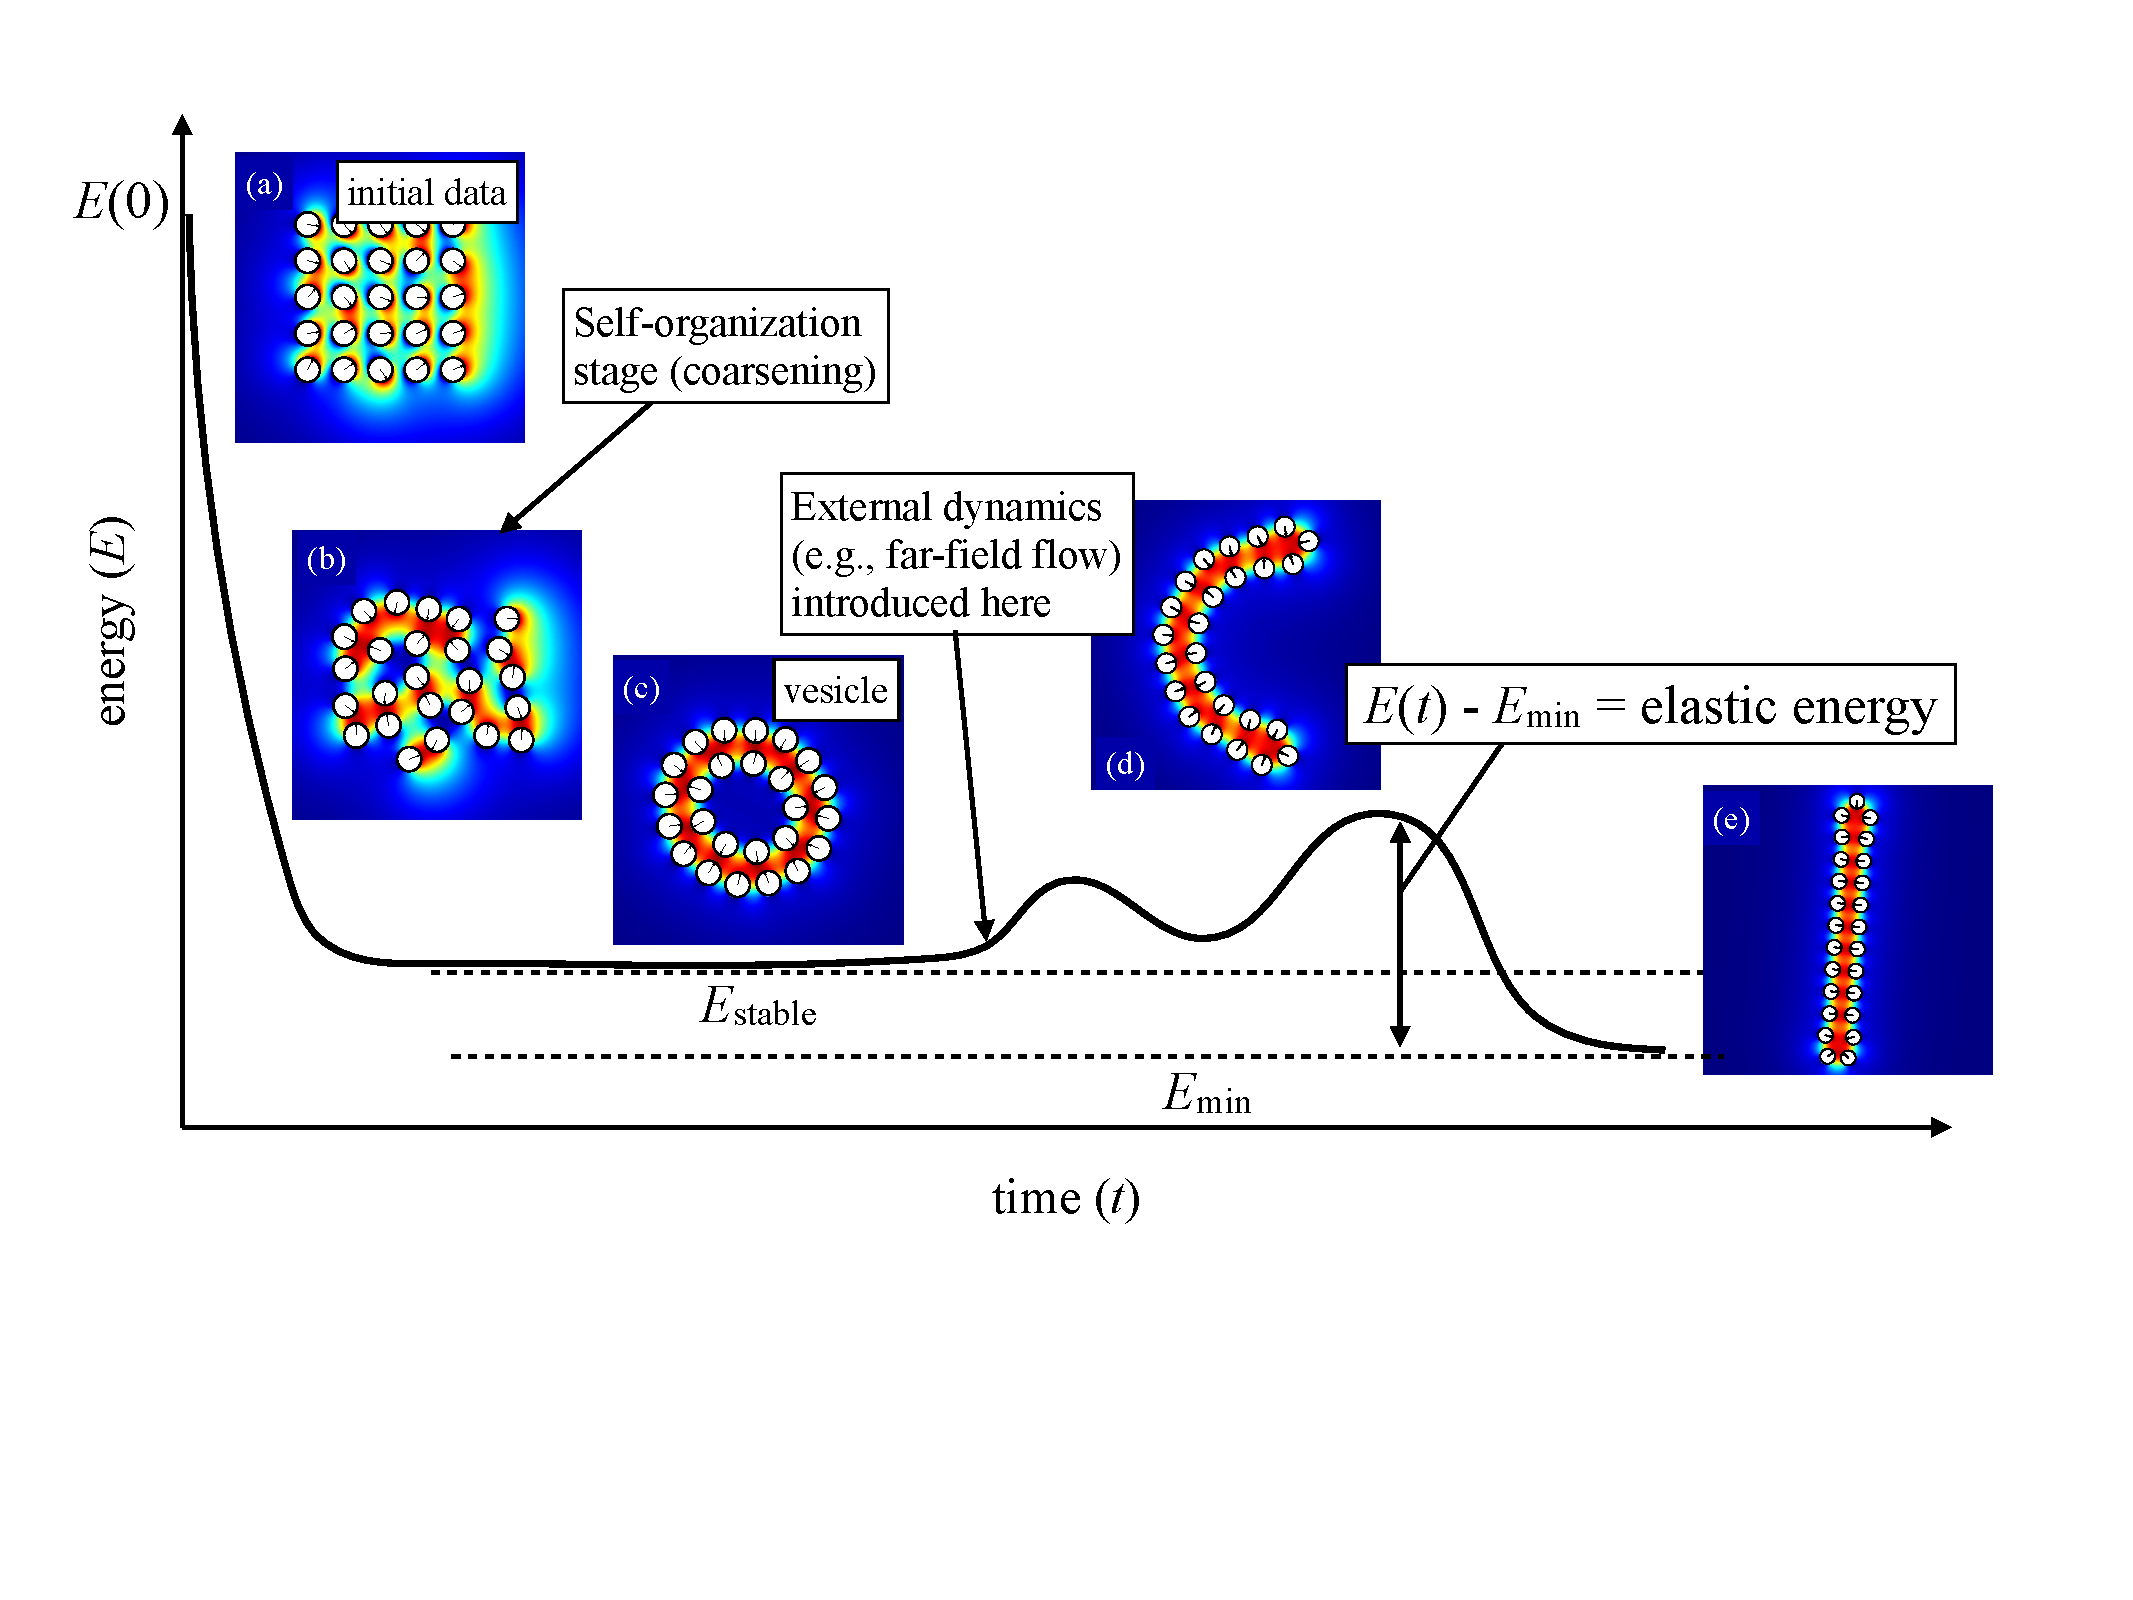
\includegraphics[width=0.9\textwidth]{figures/Background/coarsening.pdf}
\end{center}
\vspace{-20pt}
\caption{\label{fig:coarsening}
Modeling procedure.
We initilize a suspension of granules.
Under the moving domain problem
\eqref{eq:RBT}-\eqref{eqn:hydro_stress}
with amphiphilic boundary condition, the granules
self-organize into vesicle bilayers.
We then introduce external hydrodynamic effects to study elastic properties.
}
\vspace{5pt}
\end{figure}
\subsubsection{How do granule-based vesicles have an elastic energy?}
A natural question to ask is how 
elastic energy enters a formulation
coming from surface interactions like \eqref{eqn:math_motivation}.
Conceptually, random suspensions of amphiphilic
granules undergo a rapid coarsening to form bilayers.
For tens of granule, the bilayers form a single stable, ring-shaped vesicle
with energy $E_{\text{stable}}$ (Figure \ref{fig:coarsening}, (c)).
This vesicle configuration, however, is only a local minimizer,
whereas the planar configuration (Figure \ref{fig:coarsening}, (e))
is the global minimizer.  The difference between
$E(t)$ and $E_{\min}$ is the vesicle elastic energy.
Indeed, if a background flow overcomes the energy barrier to force granules apart,
then the bilayer unfolds from its circular shape into a flat shape.  

When hundreds granules are involved,
the two-dimensional granules reach an intermediate
state consisting of several bilayer segments (see Figure \ref{fig:self-assembly2}, top right).
Placing this metastable state into a mild background flow
causes the segments to join up into isolated vesicles \cite{fu-ryh-qua-you2022}.

Having a non-specific model that replicates detailed
physics and biology is the crown jewel of applied mathematics
and we believe that ours is such a model. 

\begin{wrapfigure}[11]{r}{0.5\textwidth}
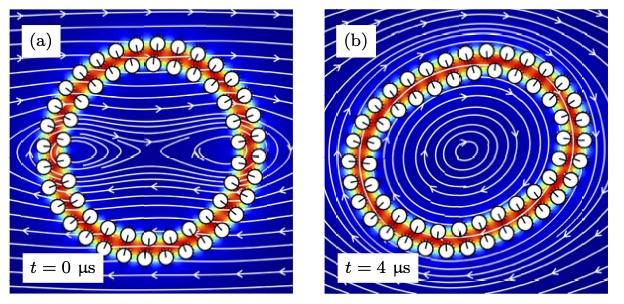
\includegraphics[width=0.5\textwidth]{figures/PreliminaryWork/TankTreading.jpg}
\caption{\label{fig:JPv_linearshear}Granular vesicles undergo
tank-treading in background shear flow.}
\end{wrapfigure}
\textit{Summary of results from the paper \cite{Fu2018_SIAM}.}
A striking aspect of the
model is its fidelity to physics.
The model contains a few
parameters; granule radius $c$,
screening length $\epsilon$,
surface tension $\gamma$.
When set to realistic values,
\cite{Fu2018_SIAM, ErLjCl89, Lin2005, Parsegian, Israelachvili80, GarciaSaez, KUZMIN2005, Petelska2012,Jackson2016},
we recover many of the well-known
elastic moduli for single-component lipid bilayers
\cite{Nagle17, Nagle17-2, LeVeWa14,NAGLE2000159}.
\emph{Bending:}


\begin{wrapfigure}[14]{l}{0.475\textwidth}
%\vspace{-10pt}
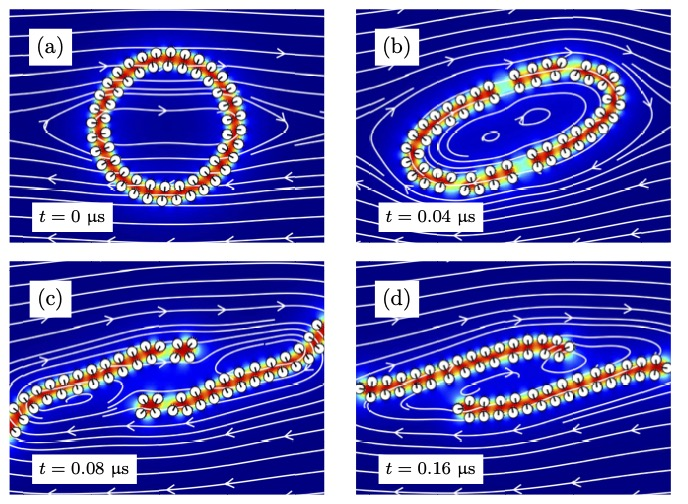
\includegraphics[width=0.475\textwidth]{figures/PreliminaryWork/Rupture.jpg}
\caption{\label{fig:JPv_rupture}Rupture of a granular vesicle under large shear rates.}
\end{wrapfigure}
\textit{Summary of results from the paper \cite{FuQuRyYo22}.}
In terms of hydrodynamics, the granule vesicles in linear
background flows \eqref{eqn:shear_BG_flow} also replicates
the behaviour of an continous, inextensible,
elastic vesicle with permeability.
The simulations showed, for the first time,
a granule-vesicle suspension behaving
as a tank-treading vesicle \cite{Finken2008, Shaqfeh11}
(see Figure \ref{fig:JPv_linearshear}).
Movies of Figure \ref{fig:JPv_linearshear} reveal
intermonolayer slip and derived values for intermonolayer
friction were in good quantitative agreement 
those derived by atomistic and Martini force field
simulation studies \cite{WuoEd06, denOtter2007, SHKULIPA2005823, Zgorski2019}.
In Figure \ref{fig:JPv_rupture},
membrane rupture occurs at large shear rates $\dot \gamma$
and we derived a dimensional scaling to 
predict critical shear rate for rupture
\cite{VLAHOVSKA2009775,keller_skalak_1982}.
Finally, a side-by-side comparison
of granule-based vesicles and the continuous model using
\eqref{eq:Canham-Helfrich} yielded shapes and trajectories that
basically overlapped.


\subsection{Outline of the proposal}
The outline of the proposal goes as follows.
Section \ref{sec:resume} describes the
PIs's expertise and prior works
in (1) membrane-fluid mechanics (2) boundary integral equations
and (3) complex fluid dynamics
that are critical to the success of this proposal. 
Section \ref{sec:proposed-work}
goes over the three specific aims of the proposal.

